\documentclass[12pt,a4paper,oneside]{article}

\setlength{\textheight}{22cm}
\setlength{\textwidth}{16cm}
\setlength{\oddsidemargin}{0cm}
\setlength{\evensidemargin}{0cm}
\setlength{\topmargin}{0cm}
\setlength{\parindent}{0cm}
\setlength{\parskip}{0.8ex}
\usepackage{listings}
\usepackage{natbib}
\usepackage{fancyhdr}
\usepackage[english]{babel}
\usepackage[utf8]{inputenc}
\usepackage[normalem]{ulem}
\usepackage{setspace}
\usepackage{url}
\usepackage{graphicx}
\usepackage{float}
\usepackage{titlesec}
\useunder{\uline}{\ul}{}
\def\code#1{\texttt{#1}}
\setcounter{secnumdepth}{4}
\renewcommand\thesection{\arabic{section}}
%\AtBeginDocument{\renewcommand{\bibname}{References}}
\begin{document}
\pagestyle{fancy}
\fancyhf{}

\title{Bachelor of Science (Hons)
\\Literature Review: Draft 1\\
Department of Computer Science\\Rhodes University\\Grahamstown
}
\author{ 
\\Author: D.G. Smith
\\Supervisor: Prof. G. C. Wells }
\date {May 2016}
\lhead{Department of Computer Science, Rhodes University, Grahamstown}
\maketitle
\begin{center}
\it{``Interprocess Communication with Java in a Microsoft Windows Environment - Heading Towards a Generic IPC design"}
\end{center}
\begin{abstract}
The purpose of this document is to survey concurrency mechanisms in the Java programming language. In addition, Microsoft Windows interprocess communication mechanisms are reviewed to implement IPC for Java on a Windows operating system. In addition, other operating system IPC mechanisms are reviewed. It also reviews general concurrency techniques which are language independent.
\end{abstract}
\pagebreak
%may need to shuffle these around and/or combine as I write
\section{Introduction}
\begin{spacing}{1.4}
Modern computing systems primarily rely on multicore processors and, as a result, parallel computing systems are now widely available \citep{garg2005concurrent}. As such, parallel programming has become an important consideration in software development since most business and consumer machines are relatively powerful and consist of multiple cores. Java is a popular object-oriented programming language that has a significant presence in the software development industry. The language at present provides a good mechanism for mulithreading programming but does not provide a significantly efficient method in which to perform interprocess communication (IPC) between Java programs running in separate Java Virtual Machines (JVMs). Current support includes distributed computing approaches such as the ``loopback" method where messages are fed to 127.0.0.1 and Remote Method Invocation (RMI)\citep{WellsIPCJava}.
\\\\
The purpose of this paper is to outline methods in which this can be implemented in a Microsoft Windows OS environment. A Linux version that has previously been implemented exists as a starting point and will be discussed later in this text. It will examine literature that is available that may aid the in the development of an enhancement to the Java programming language that will allow IPC features on a Windows operating system. This paper will also examine how the Java Native Interface (JNI) can be used as an intermediary between Java and native C code to access low-level OS IPC features. It also requires a investigation into the internal IPC mechanisms of Windows. In addition, it will provide a review of IPC mechanisms of other operating systems to aid in the design of a generic Java class library to provide the language with IPC functionality, regardless of platform or operating system.
\\\\
% maybe enum this later
Note: The term ``concurrency" within this text refers to both communication and synchronisation among processes and/or threads that belong to a particular program.
When referring to Oracle and Microsoft's API, I simply cite the top-level link to avoid a large number of references to the respective APIs.
\\\\
It it necessary to include some general background information regarding processes, threads and accepted concurrency mechanisms prior to the discussion of the techniques currently provided by the Java programming language.
\end{spacing}

\section{Processes and Interprocess Communication}
\begin{spacing}{1.4}
A process is an abstraction that is created upon program execution - it is effectively an instance of a program that is currently running within its own distinct address space \citep{modernOS}. All processes consist of three sections, namely code, data and a stack. The code section contains executable code (generally machine instructions) that the program is currently dealing with. The data section contains global variables and data that may be dynamically allocated in the heap as the program progresses through its execution stages. The stack contains any local variables that are in use. Programs that consist of a single process are known as \textit{sequential} whereas programs that consist of multiple processes (and possibly threads) are known as \textit{concurrent}. The underlying operating system (OS) is responsible for managing program processes and their subsequent threads \citep{garg2005concurrent}. Processes may also consist of implicit variables, for example the program counter as well as the contents of data registers. The state of the process may change as it executes statements \citep{trainBook}.

% confirm Understanding Linux Kernel
Different OSs generally create new processes and implement IPC in different ways, but some form of commonalities are present, such as process identifiers and synchronisation techniques. Unix-based OSs generally make use of the system call \code{fork()} to create child processes. Then additional system calls such as \code{shmget} and so forth can be used to access the native IPC mechanisms provided by the OS. In addition, Unix provides a comprehensive threading mechanism known as POSIX Threads which aid in multithreading programming \citep{linuxKernal}. An OS such as Microsoft Windows uses a function called \code{CreateProc} which handles process creation as well as features such as the process status, security and data structure access \citep{modernOS}. Further details are discussed later in this text.
\\\\
Parallel programming includes the concept of interprocess communication or IPC for short. All programs that deal with multiple processes may require a method in which to communicate to achieve the desired results. IPC can then be defined as the method in which processes (either belonging to a single program or multiple programs) pass messages to one another - i.e. process to process. This is an important concept that allows the flow of information between programs running on multicore machines \citep{modernOS}. IPC can introduce significant problems in terms of synchronisation, including mutual exclusion (race conditions) and deadlock.

% this paragraph needs work:
The Java programming model currently does not provide comprehensive support for an efficient IPC mechanism which appears to be a significant design flaw. This is particularly apparent due to the fact that multicore processing and the presence of parallel programming is almost ubiquitous in modern software engineering. Multicore central processing units (CPUs) are present in most hardware designs which also emphasises this problem. In addition, Java is a popular language that is used on many industry development jobs and this coupled with muticore processing's ubiquity adds to the problem.  
\end{spacing}

%will need to trim this section
\section{Process Synchronisation}
\begin{spacing}{1.4}
Correct synchronisation is a concept that is fundamental to concurrent program execution. It is an inherent property of IPC and is often blanketed under this term. Various languages implement synchronisation. This text will present a generic discussion of synchronisation and then proceed to sync mechanisms provided by Java, particularly within a multithreading environment.

When designing programs that access data concurrently, it is important to design them in such a way that data is consistently synchronised. This will avoid data corruption if multiple processes or threads are trying to access data that is shared \citep{garg2005concurrent}. Race conditions are anomalies that can arise when multiple processes are attempting to read or write data that is shared among them. This is a significant problem if the final result of a process depends on this data, but it was previously modified by some other arbitrary process - effectively data has been corrupted and now not relevant to the current process \citep{modernOS}. Data or a piece of code that is shared among processes, and more specifically threads, is called the \textit{critical region} or \textit{critical section}. These can include aspects such as shared resources, memory locations and other related data. In order to avoid race conditions, some form of mutual exclusion needs to be implemented in order to protect data from rogue processes that may change it in the critical region and hence alter the results of another process. It should lock the data when the program is inside of it and then release it for any other process that requires it at that point in time \citep{multithreadingwin32}. Various software-implemented synchronisation techniques exist in addition to hardware-dependent techniques. Synchronisation such as the Dining Philosophers and Producer-Consumer problems are presented. 

\subsection{Hardware Synchronisation}
In terms of hardware, synchronisation may be achieved by disabling interrupts on the CPU as soon as the process enters a critical region. This means that no process can switch into the operating system's kernel mode (i.e. context switch) and alter the region's values. When the process exits the critical region, interrupts are then re-enabled. \citep{garg2005concurrent}. This is not a feasible solution because additional problems arise. In addition, this is not possible in multicore CPU designs, as one would have to disable multiple CPU cores. Another problem that may arise by giving the CPU the ability to disable interrupts is that there is no way of telling if the CPU will re-enable interrupts at a later stage which poses significant problems to system functionality \citep{modernOS}.

\subsection{Software Synchronisation}
Software mutual exclusion can be implemented relatively easily with \textit{busy-waiting} techniques. A simple implementation makes use of lock variable that initially has a value of 0. A process subsequently tests this value to determine if a lock is in place, protecting a critical region. If the lock value is 0, a process will enter the region and set the lock to 1. An additional process can test this lock variable to determine the region's status. If the value is set, said process will wait until the region is available. This technique still has a race condition on the lock value. This can be prevented by making use of \textit{strict alternation}. This is known as a spin lock where an integer value is used to determine which process can enter the critical region. Process A will enter a critical region whilst process B continuously monitors the integer \code{turn} value \citep{modernOS}. This creates a number of significant problems as more overhead is introduced as the number of competing processes increases. In addition, other processes can be delayed by a slower process that is using the lock \citep{spinlocks1994}.

To overcome this, it is better to put competing processes to sleep to preserve CPU time. This can be illustrated by means of the Producer-Consumer problem. If a shared memory buffer exists (which can be abstracted as an array), a producer will deposit information and a producer will extract information from the buffer. Problems can arise if the consumer attempts to extract an item from an empty buffer. Conversely, a producer cannot deposit an item if the buffer is full. This can be circumvented by putting the producer and consumer to sleep until these conditions have been satisfied. As a result, \code{wakeup} and \code{sleep} are called when necessary. Problems can arise if a \code{wakeup} is made to a process that is not currently sleeping as this call will be lost.

As such, a better approach to synchronisation is to make use of semaphores, which was pioneered by \cite{dijkstraSems}. Semaphores introduce the concept of an integer \code{s} that stores a non-zero value. Once \code{s} has been given a value, only two atomic operations may be performed on them: \code{up(s)} and \code{down(s)}. \code{up} effectively means ``to release" the process whereas \code{down} means allow the process ``to pass" \citep{trainBook}. 
\end{spacing}
\begin{spacing}{1.4}
Semaphores need to ensure that the checking and subsequent changing of \code{s} is an atomic operation, therefore it is necessary to introduce a lock until the operation has been completed. It is also necessary in a multicore system. \citep{modernOS}. Semaphores are not without disadvantages including the fact that they are a low-level concept that can be prone to bugs and can be difficult to implement. If the programmer does not keep track of calls to \code{up} and \code{down}, deadlock can occur. In addition, semaphore usage can become more complicated as the complexity of accompanying algorithms increases \citep{semDisadvantages}.

% talk about monitors here
\end{spacing}	   			

%talk about shared objects and RMI
\section{Java Concurrency Mechanisms} % must be in depth
\begin{spacing}{1.4}
The Java programming language, at present, provides a significantly comprehensive support structure for multithreading programming by means of the \code{java.util.concurrent} package and \code{Thread} class. Version 5.0 of the Java platform introduced high-level APIs for concurrency in the language \citep{JavaAPI}. As such, the language provides mulithreading programming facilities through means of \code{java.lang.Thread}, methods declared as \code{synchronised} which utilise monitor concepts such as wait, notify and signal. These are described substantially in Oracle's Java API documentation, particularly within \code{java.util.concurrent}. Specifically IPC, Java currently utilises concepts such as Remote Method Invocation (RMI) which takes more of a
distributed computing approach. In addition, it can use a ``loopback" technique using 127.0.0.1 \citep{WellsIPCJava}.

\subsection{java.lang.Thread}
Java provides \code{java.lang.Thread} that allows the explicit creation of thread objects \citep{garg2005concurrent}. There are two alternative methods in which this can be utilised. Firstly, classes can be written that inherit from the \code{Thread} class, which allow the programmer to override the provided \code{run} method. Subsequently \code{start{}} can be invoked to execute the thread \citep{garg2005concurrent}. The following code adapted from \cite{JavaAPI} (the Java API) illustrates thread creation:
\end{spacing}
\begin{verbatim}
class MyThread extends Thread {
   // this method overrides the run method in Thread  
   public void run() {
      // do something
   }
   public static void main (String[] args) {
        MyThread t = new MyThread(); // create thread object
        t.start();					// launch thread
   }
}
\end{verbatim}
\begin{spacing}{1.4}
The alternative method in which to make use of Java's threading mechanism is to implement the \code{Runnable} interface. This class can then be used to implement the \code{run} method. An instance of this class is then passed into the constructor of the \code{Thread} class and then started by calling \code{start} directly, as illustrated below.
\end{spacing}
\begin{verbatim}
MyClass c = new MyClass();
new Thread(c).start();
\end{verbatim}
\begin{spacing}{1.4}
Java threads  have their local variables organised as a stack and hence can access shared variables and are generally used as lightweight processes running within the context of a single JVM \citep{trainBook}. Java threads support priority and have a minimum and maximum priority value and contain get and set methods. This can heuristically affect OS schedulers \citep{LeaConcurrentProgInJavaDesignPrinciplesPatterns}. According to \cite{HydeJavaThreadProg}, making use of Java threads can have some benefits as well as drawbacks. Benefits can include better interaction with the user, the simulation of simultaneous activities, use of multiple processors as well as performing other tasks whilst waiting for slow IO operations. Drawbacks exist, such as each \code{Thread} instantiation, which introduces overhead and use of memory resources. They also require processor resources such as starting, scheduling, stopping and killing of \code{Thread} objects. According to \cite{JavaAPI}, Java concurrency mostly concerns itself with threads as opposed to multiple processes. In addition, most instances of the JVM run as a single process with associated child threads as units of execution. This is a distinct concept from that of IPC between Java processes belonging to separate JVMs.  

\subsection{java.util.concurrent}
The package \code{java.util.concurrent} (which is affiliated with \code{Thread}) provides concurrency classes that include synchronisation mechanisms that contain operations that set and inspect thread state, various mutual exclusion solutions as well as barriers and queues and so forth \citep{Lea_java.util.concurrent}. These facilities are sufficient for developing good multithreaded applications which aim to eliminate problems that can arise such as deadlock, race conditions and unintentional thread interaction \citep{WellsEfficientIPCJava}. 
\\\\
\cite{JavaAPI} provides tools such as concurrent data structures like  \code{ConcurrentLinkedQueue<E>} which contains methods such as \code{peek}, \code{poll} and so forth which allows threads to access concurrent data. The \code{Executor} interface is a framework that essentially allows the creation of custom thread-like systems and for defining lightweight task frameworks.

In terms of synchronisation, the package offers \code{Semaphore}, \code{CountDownLatch}, \code{CyclicBarrier}, \code{Phaser} and \code{Exchanger}. 

\subsubsection{Semaphore}
The \code{Semaphore} class in Java is implemented in the form of a counting semaphore which keeps track of a set of permits. The method \code{acquire} tries to gain access to a resource but blocks if a permit is unavailable. Conversely the method \code{release} adds a permit to a resource. Permits are kept tracked of in the form of a simple integer counter. The constructor accepts a fairness parameter which ensures that no thread starvation occurs if it tries to acquire a resource but is continually blocked \citep{JavaAPI}.

\subsubsection{CountDownLatch}
This essentially introduces a lock until another thread completes its operations. The object is given a count and the method \code{await} blocks until the count reaches zero. \code{countDown()} decrements the count on each invocation. Subsequently threads are released. This class can be used as an on or off latch by giving it a count of one \citep{JavaAPI}.

\subsubsection{CyclicBarrier}
This class implements barrier functionality that allows for groups of threads to catch up to a certain point before proceeding and is cyclic in nature since the barrier can be reused once the waiting threads are released \citep{JavaAPI}.

\subsubsection{Phaser}
This barrier technique is very similar to \code{CyclicBarrier} but allows a flexible addition of threads to be added at any time (unlike \code{CyclicBarrier}. A simple method called \code{register()} can be invoked to add a task. A phase number is initially generated and increases to a maximum number previously defined once all tasks reach the phaser number. It is wrapped around once the count reaches the maximum number. Phasers support a concept known as \textit{Tiering} that allows subphasers to be created, which can reduce the amount of contention if there are a large number of tasks \cite{JavaAPI}.

\subsubsection{Exchanger}
This defines a point at which threads can pair together and exchange elements. On entry, threads pair and exchange their partner's object. This is performed within the \code{exchange()} method \citep{JavaAPI}. 
\\\\
The mechanisms provided by \code{java.util.concurrent} ultimately require a shared address space for JVM threads to synchronise and have common access to shared objects \citep{WellsIPCMultiProc}.
\end{spacing}
\subsection{IPC}
% RMI, loopback, shared objects, CORBA
\begin{spacing}{1.4}
Current Java IPC mechanisms appear to make use of distributed programming features such as the ``loopback" mechanism, remote method invocation (RMI) and the Java Message Service (JMS).
\end{spacing}
\subsubsection{Loopback Mechanism}
\begin{spacing}{1.4}
According to \cite{WellsIPCJava}, Java provides a robust mechanism for communication in terms of distributed computing using the Internet Protocol's (IP) loopback system using 127.0.0.1. This means that communication can take place between multiple processes on a single machine. This takes the form of socket programming using TCP/UDP by using Java's standard socket API \citep{taboada2013javaforHPC}. Messages can be encapsulated into packets and passed into the IP stack as necessary. Messages can then passed to programs running in separate JVMs using this loopback mechanism, thereby providing a form of IPC. \cite{taboada2013javaforHPC} states that Java's network support over TCP/UDP tends to be an ineffient communication mechanism. In addition, research conducted by \cite{WellsIPCMultiProc} also found it to be inefficient. This was due to messages having to traverse the protocol stack. It also broke Java's write once, run anywhere (WORA) principle since native code was used. 
\end{spacing}
\subsubsection{Remote Method Invocation}
% RMI
\begin{spacing}{1.4}
Remote Method Invocation (RMI) allows methods to be called in an object that are running within the context of another JVM. Arguments of the called method are packetised and sent over a network to a JVM. They are then passed into the remote method as necessary. The object to which the remote method belongs should provide safety mechanisms as the caller does not know about the callee's state \citep{JavaConcurrencyInPractice}. RMI is used in conjunction with the loopback method discussed above. A similar mechanism known as Common Object Request Broker Architecture (CORBA) also involves the remote calling of methods to provide a distributed solution \citep{WellsIPCMultiProc}. Yet another form of distributed communication is the Java Message Service (JMI) which provides communication between applications \citep{JavaAPI}. RMI provides a solution to IPC but according to \cite{taboada2013javaforHPC}, at a cost of poor performance.
\\\\
It should be emphasised that the current facilities in Java are inherently thread-based as opposed to IPC-based. The current network communication mechanism through the IP stack has significant overhead.
\end{spacing}
\section{Java Native Interface}
% can talk about some of the params that are used
\begin{spacing}{1.4}
The Java Native Interface (JNI) is a framework, released in 1997 in JDK 1.1, that allows the integration of native code into standard Java applications. Currently JNI supports C and C++ within its framework. It can be used to integrate legacy code with Java applications as well as allow the language to invoke native code and the other way around. JNI can invoke native methods that are written as functions in a native language, such as C or C++. These native functions reside in native libraries (i.e. on a Windows platform as .dll files). JNI can also embed a JVM into applications writen in a native language. There are two significant implications of using JNI. Firstly, since native code is being used, it breaks Java's property of “write once, run anywhere”. This means that code written will be host dependent. Therefore a recompile would be necessary if this code was to be ported to another host environment. Secondly, Java is type safe and protects the programmer whereas C and C++ does not \citep{LiangJNISpecification}. JNI allows access to low-level machine features such as memory, IO and so forth, including IPC facilities \citep{IBM2009}. \cite{LiangJNISpecification} states that prior to using JNI, other mechanisms should be considered such as other IPC mechanisms, legacy databases and other Java distributed object technologies.
\subsection{How It Works}
Methods are declared as \code{native} in Java. This means that their implementation is then written in a native language such as C/C++. Once this code is compiled and fed into \code{javah}, a C header file is generated with the native method's function prototype. This function can then be written in C/C++ and compiled using any standard C compiler (e.g. gcc, cc, cl, Borland C++ and so on). In a Windows environment, a .dll shared library file is created and linked into the Java program that is calling the native code. The function generated by \code{javah} may resemble the following:
\begin{verbatim}
JNIEXPORT jstring JNICALL Java Sample1 stringMethod
  (JNIEnv *, jobject, jstring);
\end{verbatim}
\code{JNIEXPORT} and \code{JNICALL} are macros that ensure that the function is exported from \code{jni.h} which is a native library provided by the Java platform. \code{jstring} means that the function is typed and returns a string. The parameter \code{JNIEnv *} points to a pointer that in turn points to a function table (an array-like structure). The function table contains pointers that point to native functions that have been written. The image below is adapted from \cite{LiangJNISpecification}.
\begin{figure}[H]
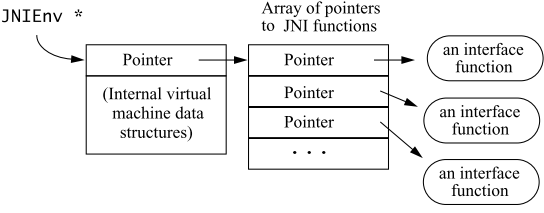
\includegraphics[width=12cm]{jni_function_table}
\caption{JNI function table}
\end{figure}
\code{jobject} refers to the object that the method belongs. If it is a static method, it is a reference to the class that it belongs to. The \code{jstring} parameter is an argument given to the function in the Java code. In this case, it was a string passed into the method. There can be any arbitrary amount of arguments passed into the function and will be reflected here when the C/C++ function types are generated \citep{LiangJNISpecification}.
\subsection{Performance}
According to \cite{IBM2009} and \cite{WellsIPCMultiProc}, use of the JNI can incur performance penalties. Performance is somewhat restricted when calls to native code are made or when a JVM has to move up a class hierarchy. This is true if a native function attempts to call a method written in Java.
\end{spacing} 
\section{Linux Implementation}

\begin{spacing}{1.4}
\subsection{Initial Implementation}
A Linux and Solaris-based
implementation was created by \cite{WellsIPCMultiProc} using Unix
System V calls. The approach taken was to develop Java classes using JNI
to access these system calls. The Unix IPC features used included
message queues, semaphores, shared memory and piping. The
implementation aimed to make the native Java methods as close to
possible as the system calls. This includes names and parameter lists.

\subsubsection{Problems Encountered}
Problems encountered by \cite{WellsIPCMultiProc} was the
difference in data representation between Java and C. Data representation
issues arrised in aspects such as error handling (i.e. exceptions vs -1
returns), control system calls, semaphore operations and shared memory.
Results

\subsubsection{Results}
Simple communication was peformed and and
compared against the network loopback connection. It was found that all
the Unix System V IPC mechanisms were significantly faster than using the
loopback method. Named pipes were found to be fastest since it made
minimal use of JNI calls. This was the case for tests running on Ubuntu
8.05.1 and Solaris.

\subsection{Shared Memory Object Framework Model}
The intial implementation by \cite{WellsIPCMultiProc} contained some
portabilty inssues here since calls to native code were being made. A
Shared Memory Object Framework was developed by \cite{WellsEfficientIPCJava} that aimed to create a more abstract solution to Java's IPC problems.
% continue talking here...
\end{spacing}

\section{Windows IPC and Concurrency Mechanisms}  % must be in depth
\begin{spacing}{1.4}
Modern Microsoft Windows Operating Systems appear to be highly modular in nature, with emphasis on object-oriented design which is illustrated by the following diagram adapted from \cite{WinInt2009}.
\begin{figure}[H]
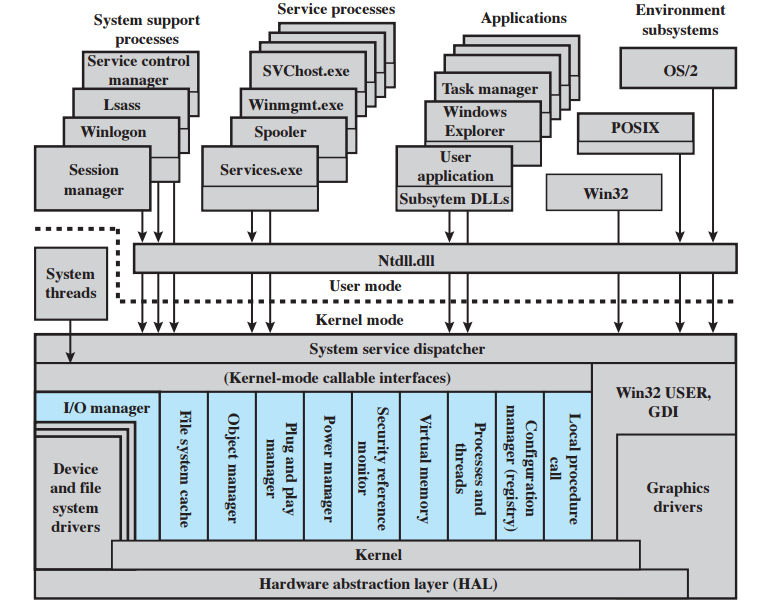
\includegraphics[width=10cm]{winArch} % will need to be scaled after text has been 
\label{fig:winArch}
\caption{Windows System Architecture}
\end{figure}
According to \cite{OSInternals&DesignPrinciplesStallings}, the Windows kernel mode is divided into the following blocks: executive, kernel, the hardware abstraction layer, device drivers and the windowing and graphics system as depicted in figure 2 above.

\subsection{Windows Executive}
The Executive block contains the base services such as memory, thread management and IPC. The kernel block handles process switching and thread scheduling. 
It provides an application programming interface (API) for user mode software \citep{OSInternals&DesignPrinciplesStallings}. Within the Executive block, several other modules are built in. The module specific to IPC is the Process/thread manager. This module is responsible for creating, managing, and deletion of processes and associated threads. The Executive also contains a module called Local Procedure Call (LPC) that allows local processes to communicate. It is similar to remote procedure calls (RPC) \citep{OSInternals&DesignPrinciplesStallings}. The executive contains functions that are callable from user-mode through the Windows API \citep{WinInternalsPart12012}.

\subsection{The Windows Process}
Windows processes are defined as objects that have a number of attributes and functions (shown in figure 3) and contains at least one thread. These threads may execute in parallel on multicore systems. \citep{OSInternals&DesignPrinciplesStallings}.

\begin{figure}[H]
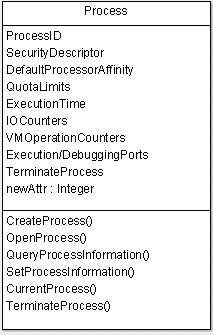
\includegraphics{procObj}
\label{fig:procObj}
\caption{A Windows process object. Adapted from \cite{OSInternals&DesignPrinciplesStallings} p. 187} 
\end{figure}

\subsubsection{CreateProcess()}
The \code{CreateProcess()} function creates a process and its primary thread. The function takes the following parameters. The application name, command line to be executed, process attributes, thread attributes, inherit handles, creation flags, a pointer to the environment block, the current directory, start up information and current process information. The resulting process is assigned an identifier and is valid until termination. \code{TerminateProcess()} can be used to the kill the process by passing in the correct handle to the process that needs to be exited. Additional functions exist in the Windows API that complement this function and include functionality such as returning handles, opening processes, returning process information and so forth \citep{MSDN_API}.

\subsection{Windows' Client/Server Model}
Windows' services, subsystems and IPC mechanisms are structured according to a client/server model of computing which aims to simplify the Executive, improve reliability and provide a base for distributed computing \citep{OSInternals&DesignPrinciplesStallings}. Windows' IPC mechanism are abstracted by means of this model where a client is a process that requests data from another process. A server responds to such requests. \citep{MSDN_IPCExplanation}. The following subsection discusses how applications can communicate.
\subsection{Process Communication Mechanisms}
Windows provides the following IPC mechanisms as per the APIs provided by Microsoft (Windows API).
\subsubsection{Clipboard}
The clipboard acts as a depository which allows applications to share data. An application deposits data into the clipboard which another application can later retrieve in a format it understands. Applications can be running on the same machine or across a network \citep{MSDN_IPCExplanation}.

Key functions such as \code{OpenClipboard}, \code{EmptyClipboard}, \code{SetClipboardData}, \code{CloseClipboard} and \code{GetClipboardData} are used \citep{IPCWindowsLinkedInSlides}. \code{SetClipboardData} deposits data on the clipboard in a particular format. \code{GetClipboardData} retrieves data from the clipboard in the format specified \citep{MSDN_API}.
\subsubsection{Component Object Model (COM)}
The Component Object Model can be used to create software components that can interact. According to \cite{MSDN_API}, it is a standard that defines how COM objects interact with other objects. Objects can reside in a single process or in multiple other processes. COM objects can access data and an object's data through a set of functions known as interfaces. The functions that are part of the interface are known as methods. Interface methods are accessed through a pointer to that interface. Common functions exist between all COM objects; i.e. they are mandatory functions that all components require.
\subsubsection{Data Copy}
By making use of \code{WMCOPYDATA} that is part of Windows Messaging, an application can send data to another application. In order to use data copying, the receiving process needs to be aware of the format of the data being sent as well as identity of the sending process. Data can be encapsulated within a private data structure. It can be sent to the receiving application along with the a pointer to the data structure using \code{WMCOPYDATA} \citep{MSDN_API}.
\subsubsection{Dynamic Data Exchange (DDE)}
\cite{MSDN_API} defines DDE as an extention of the Clipboard as it makes use of the same formats. Data can be exchanged at an ongoing rate, or as new data becomes available. \cite{MSDN_API} desribes DDE as not as efficient as newer IPC mechanisms. Its important to note that the DDE makes use of shared memory to exchange data between appilcations.

DDE contains a .dll file called Dynamic Data Exchange Management Library (DDEML) that processes can use to share data. The library provides functions and messages that adds DDE to applications. DDEML makes use of a conversation concept that makes it easier for the programmer to manage messages; pointers and atoms to shared memory are replaced by making use of string handles. In addition, DDEML forces applications to implement DDE in a consistent fashion. Programs should have the DDEML header file within its source code \citep{MSDN_API}.

A DDE client can start a conversation with a DDE server and can participate in multiple conversations simultaneously. A process can be a client or a server as necessary. DDE conversations are identified by the process/application name and a ``topic". The topic represents the data that is to be exchanged between processes \citep{MSDN_API}.

\subsubsection{File Mapping}
File mapping allows a process to see the contents of a file as a block of memory within its own address space. This is essentially a form of shared memory. Pointer operations are used to access and modify contents of the mapped file with some form of synchronisation mechanism (such as a semaphore) used to prevent corruption and maintain the file's consistency. This IPC technique can only work on a single machine and the file cannot exist on a remote computer \citep{MSDN_API}.

\cite{IPCWindowsLinkedInSlides} states that a file mapping can be created by using the function \code{CreateFileMapping}. The file map view is then put into address space of the current process by using \code{MapViewOfFile}. \code{CopyMemory} is then used to write messages to the view. File mappings are closed using \code{UnmapViewOfFile} and \code{CloseHandle}. A client process can examine the contents of the mapping using \code{OpenFileMapping} and put the view into its address space by calling \code{MapViewOfFile}. It can also close mappings as necessary.

\subsubsection{Mailslots}
Windows Mailslots follow the client-server model with one-way process communication. A server process will create a Mailslot and the client can write messages into the Mailslot as required. The messages are saved within the Mailslot until read. Messages can be sent on a local host or across a network. Message size is only limited by what the server specifies when the slot is created \citep{MSDN_API}. 

Mailslot messages follow a datagram format and as such, no guarantees are made in terms of receipt. Mailslots receive a handle when created and is used when the process that created it accesses data within it. A process that is aware of a Mailslot's existence can insert a message there. Mailslots also have a broadcasting capability where each process can create a slot and all participating processes can deposit their messages to the respective Mailslots that exist. This means that a Mailslot can be a server and client which can allow two-way communication \citep{MSDN_API}.

Mailslots can be created using \code{CreateMailslot()} and its contents examined using \code{ReadMailslot()}. A number of auxiliary functions exist such as \code{GetMailslotInfo()} and so forth. Handles can be closed using \code{CloseHandle()}. Clients can create a file and write to the slot using \code{CreateFile()} and \code{WriteFile()}/\code{WriteMailslot()} \citep{IPCWindowsLinkedInSlides}.

\subsubsection{Pipes}
Windows uses two types of pipes for IPC: anonymous and named pipes.

Anonymous pipes only allow related processes to exchange data and cannot be used over a network. They are typically used to exchange data between parent and child processes by using read and write handles respectively. \code{CreatePipe()} returns read and write handles for an anonymous pipe and specifies a buffer size. These handles are passed to another process to communicate, usually by means of inheritance where the handle is passed from the parent (server) process to the child (client) process. The relevant handle is sent depending on whether a read or write operation must occur. \code{ReadFile()} is used to read from the pipe and conversely \code{WriteFile()} is used to write to the pipe. \code{CloseHandle()} closes a process's pipe `connection' \citep{MSDN_API}. Asynchrony is not supported by anonymous pipes \citep{lewandowski1997interprocess}.

According to \cite{MSDN_API}, named pipes can be used between unrelated processes and across a network. Processes can act as a server or client without having to create multiple anonymous pipes. \code{CreateNamedPipe()} and \code{ConnectNamedPipe()} are used by the server and client respectively. Standard \code{ReadFile()} and \code{WriteFile()} functions read and write to the pipe as necessary. 

\subsubsection{Remote Procedure Call (RPC)}
Similar to RMI discussed above, RPC allows procedures to be called remotely, either on a local machine or across a network. \cite{MSDN_API} states RPC conforms to the Open Software Foundation's (OSF) Distributed Computing Environment (DCE) which allows RPC to work on other OSs that support DCE.

\subsubsection{Windows Sockets (Winsock 2)}
Winsock creates a channel between communicating processes and is protocol independent with asynchronous communication capabilities \citep{lewandowski1997interprocess}. Socket handles can be treated as a file with usual I/O operations \citep{MSDN_API}.

Data communicated by processes can be stream-based in the form of bytes or packetised in the form datagrams but no quality of service is guaranteed \citep{IPCWindowsLinkedInSlides}. In terms of local IPC, localhost can be used to send and receive data, as long as the correct IP addresses are specified.

\subsection{Windows Interprocess Synchronisation}
The Windows API provides functions that allow processes to synchronise as necessary. This is particularly important with regards to shared memory when there is competition for resources. Functions such \code{CreateEvent()}, \code{CreateSemaphore()}, \code{CreateMutex()} among others return handles that processes can use for the same event. These are generally used in conjunction with the security parameter defined in \code{CreateProcess()} \citep{MSDN_API}.
\end{spacing}

\section{Summary}
\begin{spacing}{1.4}
The current trend of multicore computing emphasises the significance of parallelism, multithreading and communication in general \citep{taboada2013javaforHPC}. 

Investigation of Java's concurrency mechanisms found that the language is heavily thread oriented and that it provides a good mechanism for multithreading programming. Opposed to this is the language's lack of communication between separate JVM processes. 

The existing Linux and Solaris implementation that used JNI to provide Java with IPC was successful and proved that a more efficient method of IPC could be developed without using the loopback method and ``clunky" socket programming. The review of the use of JNI highlighted a few efficiency problems with calls to native code, therefore calls to JNI should be as limited as possible. In addition, the SMOF proved that portability issues can be addressed, but it may limit IPC communication to shared memory. As such, use of common IPC features among different OSs should be taken into account when developing generic version of the Java class library.

Windows provides a fairly comprehensive set of IPC mechanisms that can be integrated with Java processes, albeit at the cost of complexity when compared to Unix system calls. 
\end{spacing}
\pagebreak
% MUST PUT IN LOCATION OF PUBLICATIONS
\bibliographystyle{apa}  

\bibliography{refs2}  

\end{document}




